
 		\begin{figure}
 			\centering
 			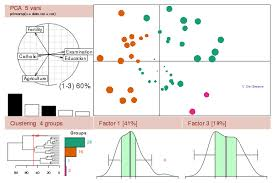
\includegraphics[width=0.97\linewidth]{CRAN}
 			\caption{Comprehensive R Archive Network}
 			
 		\end{figure}
 		
 		

 		\frametitle{R Packages}
 		
 		\begin{itemize}
 			\item ``10 R packages I wish I knew about earlier" - Drew Conway (Yhat.com, February 2013)
 			\bigskip \item ``The HadleyVerse" - Hadley Wickham
 			\begin{itemize}
 				
 				\item  ggplot2, dplyr, reshape, lubridate, stringr
 				
 				\item  With Romain Francois, Dianne Cook and Garret Grolemund.
 			\end{itemize}
 			\bigskip
 			\item Dr Brendan Haplin (UL): lme4 ,TraMineR, Gelman's arm, MASS, foreign. 
 			\bigskip
 			\item Shiny - Web Applications with \texttt{R}
 		\end{itemize}

 		
 		
 		
 		Some examples of packages are Actuar, written for actuarial science, and
 		QRMlib, which complements the Quantitative Risk Management The command library()
 		lists all the available packages. 
 		
 		To load a particular package, for example MASS, we would
 		write
 		library(MASS)
 		
<p>

 		
 		\frametitle{Packages}
 		\begin{itemize}
 			\item The CRAN package repository features 6107 available packages. 
 			\item Packages contain
 			various functions and data sets for numerous purposes, e.g.
 			\textbf{\textit{ggplot2}} package, \textbf{\textit{AER}} package, \textbf{\textit{survival}} package, etc.
 			\item Some packages are part of the basic installation. Others can be
 			downloaded from CRAN.
 			\item To access all of the functions and data sets in a particular package,
 			it must be loaded into the workspace. 
 			\item For example, to load the
 			\textbf{\textit{ggplot2}} package:
 		\end{itemize}
 		\begin{framed}
 			\begin{verbatim}
 			install.packages(ggplot2)
 			library(ggplot2)
 			\end{verbatim}
 		\end{framed}
<p>

 		\frametitle{4.2 Using and Installing packages}
 		\begin{itemize}
 			\item Many packages come with R. To use them in an R session, you need to load the package, as
 			previously demonstrated.
 			\item Some packages are not automatically installed when you install R but they need to be downloaded
 			and installed individually. 
 			\item We must first install them using the install.packages()
 			function, which typically downloads the package from CRAN and installs it for use. (follow the
 			instructions as indicated).
 		\end{itemize}
<p>

 		\begin{framed}
 			\begin{verbatim}
 			install.packages("ggplot2")
 			install.packages("qcc")
 			install.packages("sqldf")
 			install.packages("RMongo")
 			install.packages("randomforest")
 			\end{verbatim}
 		\end{framed}
 		
<p>

 		\frametitle{4.2.1 Version of R}
 		Many packages will require you to have the most recent version of R and also other packages.
 		It is a good idea to update regularly.

<p>

 
